\reportheading{4. Air distribution at 40\% flow (Task 2)}
\subhead{4.1 Minimum flow and catalogue interpolation}
The VAV minimum for each outlet is set at 40\% of its own peak allocation, reducing the total supply to 5236.526 L/s. Although the diffuser size and characteristic lengths remain unchanged, the throw changes with flow. These operating values for every outlet are provided in Appendix A.

South of SD-60, the minimum supply is 0.40 × 137.76 = 55.104 L/s. The 8-inch catalogue gives throws of 1.5 m and 2.9 m at 33 L/s and 66 L/s, so linear interpolation gives $1.5+\frac{(55.104-33)(2.9-1.5)}{33}=2.438$ m. With L = 2.100 m, the unrounded ratio is 1.1608, which is the lowest of the minimum-flow directions.

A proportional reduction in airflow does not produce the same percentage drop in throw. At SD-60, the peak flow of 137.76 L/s lies between the 132 and 165 L/s catalogue rows and gives about 4.27 m of throw. However, reducing the airflow to 40\% leaves about 57\% of this peak throw. Scaling the peak throw directly by 0.40 would give only 1.71 m and would reverse the conclusion for the 2.10 m southward path. Therefore, a second catalogue interpolation is used for every outlet in the minimum condition.

\subhead{4.2 Interpretation across the operating range}
Minimum-flow directional ratios range from 1.1608 to 2.1437 and satisfy the target selection interval. However, the controlling location changes as the VAV boxes throttle. At peak flow, the two wing outlets discharge towards a midpoint only 1.500 m away, whereas at minimum flow, SD-60 still needs to supply 2.100 m to the south. As a result, a smaller low-flow margin is left due to its 2.438 m catalogue throw, in comparison with other directions (Figure 2).
{\centering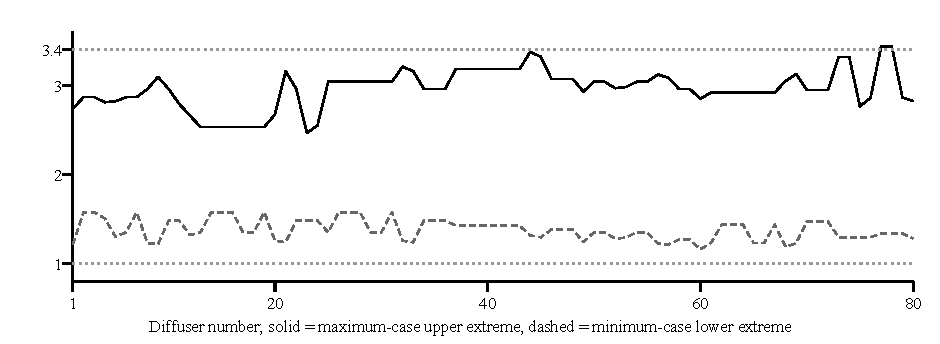
\includegraphics[width=\linewidth]{figures/diffuser-selection.pdf}\par}
\reportfigure{}{Figure 2. Peak upper and minimum-flow lower directional ratios by diffuser.}
The ASHRAE selection table shown in the course design guide applies the 1.0–3.4 interval to a louvered ceiling diffuser for cooling loads between 35 and 160 W/m². Assuming the sensible cooling load is directly proportional to the airflow, the minimum load is 68.04 W/m², whereas the peak load of 170.1 W/m² is above the table range, making the peak comparison serve only as a guide, as stated in Appendix E's separate manufacturer assessment. In practice, the point of interest at low flow is the end of the longer paths, and for SD-60, the catalogue throw is about 0.34 m longer than the southern reference distance. Conversely, at peak load, the concern shifts to the overlapping jets due to the facing outlets in the wing.
